\documentclass[12pt]{article}
\newcommand\tab[1][.7cm]{\hspace*{#1}}
\usepackage{amsmath}
\usepackage{amsfonts}
\newcommand*\diff{\mathop{}\!\mathrm{d}}
\newcommand*\Diff[1]{\mathop{}\!\mathrm{d^#1}}

\usepackage{graphicx}
\graphicspath{ {images/} }

\usepackage{listingsutf8}
\usepackage[a4paper, total={16cm, 23.7cm}]{geometry}
\DeclareMathSizes{12}{13}{10}{8}
\setlength\parindent{0pt}

% !TeX spellcheck = en_US

\begin{document}
	
	
	\begin{center}
	\Huge Applied FEM\\		
	Assignment\\
	Peter Kardos
	\end{center}
	\vspace{.5pc}	
	
	\iffalse
	\section*{\large Part A}
	\vspace{.5pc}
	
	
	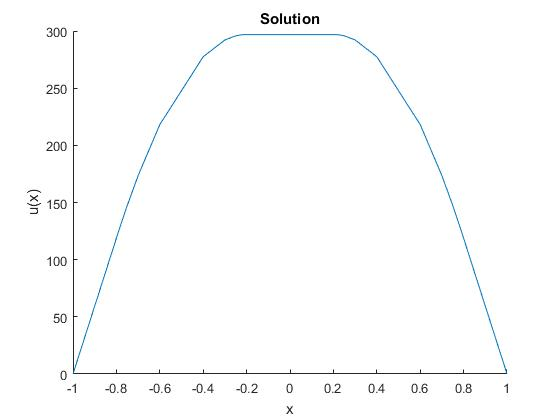
\includegraphics[width=\textwidth]{p1_solution}
	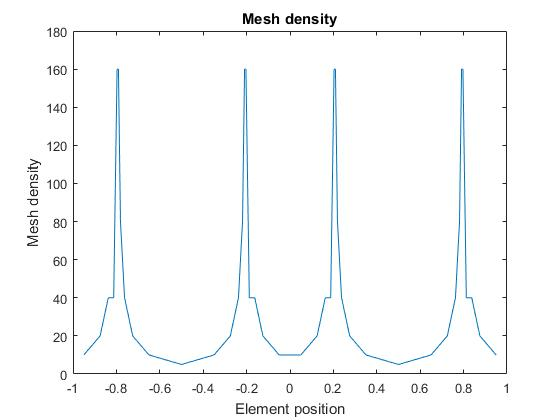
\includegraphics[width=\textwidth]{p1_dens}
	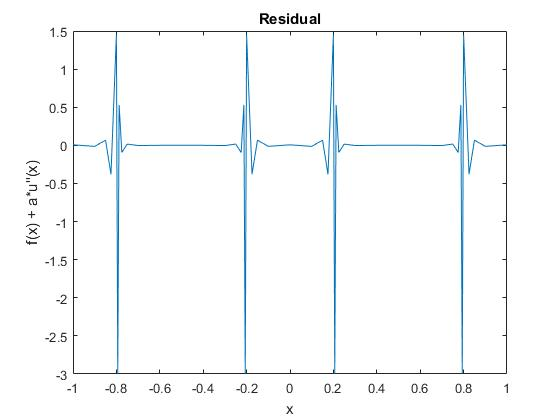
\includegraphics[width=\textwidth]{p1_resid}
	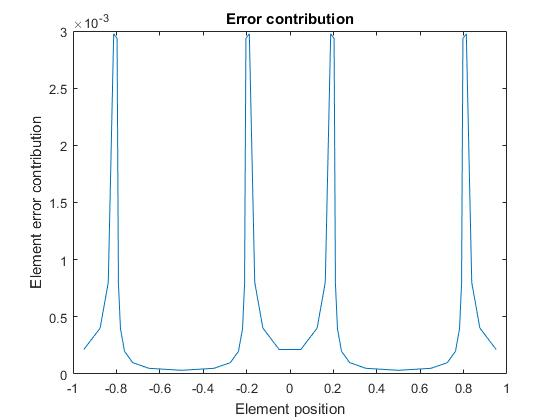
\includegraphics[width=\textwidth]{p1_errind}
	
	
	\newpage
	\large{task1.m}
 	\normalsize
	\lstinputlisting[breaklines=true]{Part1/task1.m}
	
	
	\newpage
	\large{fem\_adaptive\_solver.m}
	\normalsize
	\lstinputlisting[breaklines=true]{Part1/fem_adaptive_solver.m}
	
	
	\newpage
	\large{fem\_solver.m}
	\normalsize	
	\lstinputlisting[breaklines=true]{Part1/fem_solver.m}
	
	
	\newpage
	\large{load\_vector.m}
	\normalsize	
	\lstinputlisting[breaklines=true]{Part1/load_vector.m}
	
	
	\newpage
	\large{stiffness\_matrix\_ddu.m}
	\normalsize	
	\lstinputlisting[breaklines=true]{Part1/stiffness_matrix_ddu.m}
	
		
	
	\newpage
	\fi
	\section*{\large Part B}
	\vspace{.5pc}
	
	\large Part1 graphs
	
	
	\normalsize
	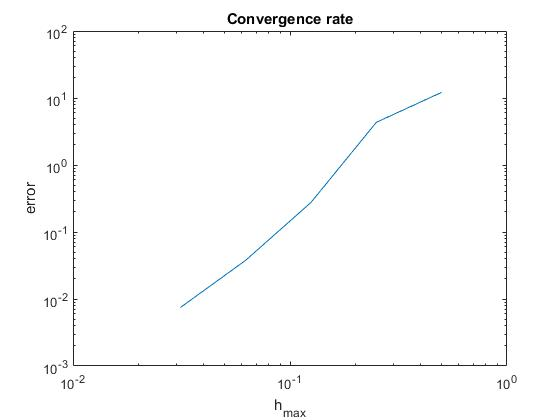
\includegraphics[width=\textwidth]{p2_1_convrate}
	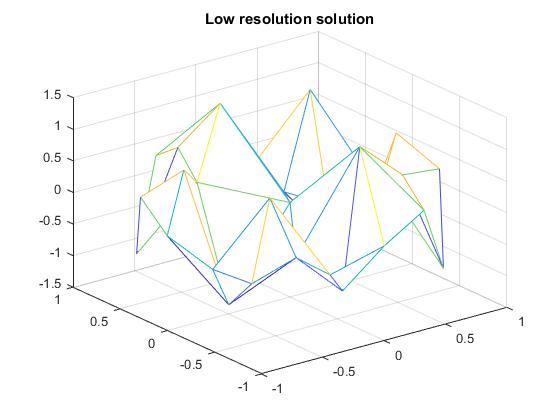
\includegraphics[width=\textwidth]{p2_1_lowres}
	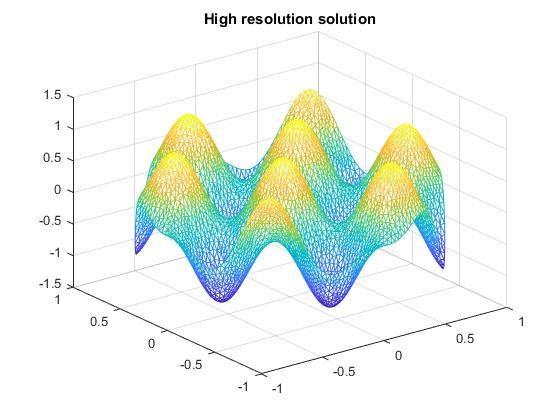
\includegraphics[width=\textwidth]{p2_1_highres}
	
	
	\newpage
	\large Part2 graphs
	
	
	\normalsize
	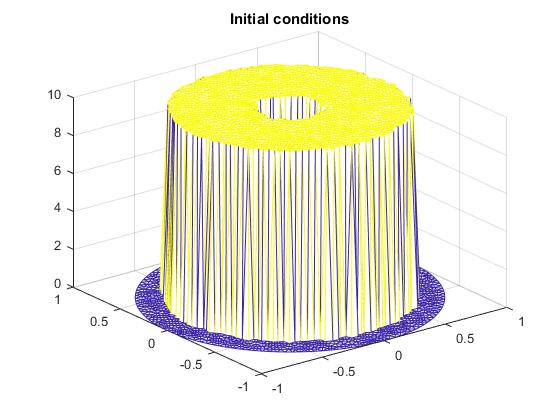
\includegraphics[width=\textwidth]{p2_2_init}
	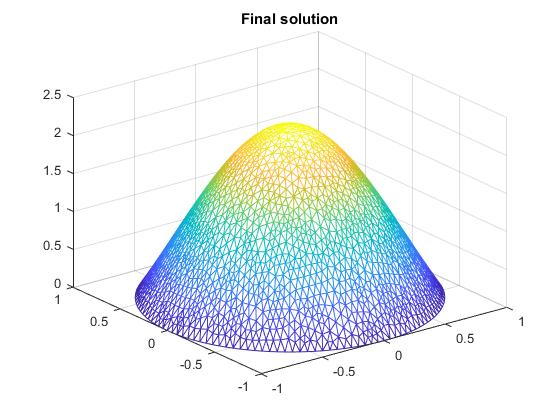
\includegraphics[width=\textwidth]{p2_2_final}
	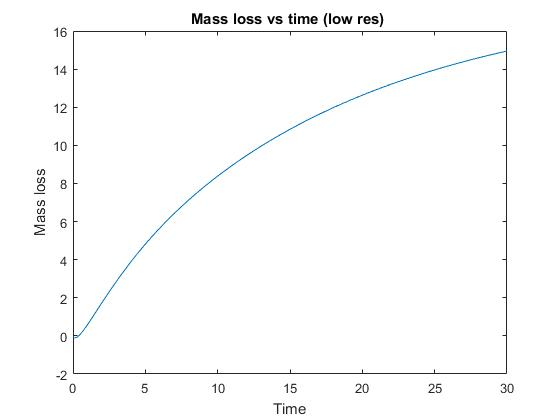
\includegraphics[width=\textwidth]{p2_2_mllow}
	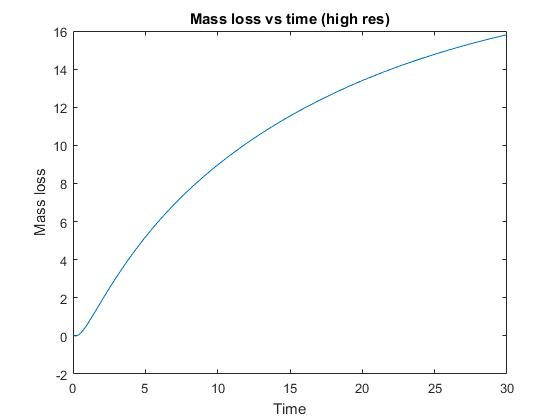
\includegraphics[width=\textwidth]{p2_2_mlhigh}
	
	\newpage
	\large{task2\_p1.m}
	\normalsize
	\lstinputlisting[breaklines=true]{Part2/task2_p1.m}	
	
	\newpage
	\large{task2\_p2.m}
	\normalsize
	\lstinputlisting[breaklines=true]{Part2/task2_p2.m}	
	
	\newpage
	\large{get\_element\_transform.m}
	\normalsize	
	\lstinputlisting[breaklines=true]{Part2/get_element_transform.m}	
	
	\newpage
	\large{load\_vector.m}
	\normalsize	
	\lstinputlisting[breaklines=true]{Part2/load_vector.m}	
	
	\newpage
	\large{mass\_loss.m}
	\normalsize	
	\lstinputlisting[breaklines=true]{Part2/mass_loss.m}
	
	\newpage
	\large{mass\_matrix.m}
	\normalsize	
	\lstinputlisting[breaklines=true]{Part2/mass_matrix.m}
	
	\newpage
	\large{stiffness\_matrix.m}
	\normalsize	
	\lstinputlisting[breaklines=true]{Part2/stiffness_matrix.m}
	
	\newpage
	\large{unit\_phi\_mc.m}
	\normalsize	
	\lstinputlisting[breaklines=true]{Part2/unit_phi_mc.m}
	
	
\end{document}